%TODO 制作导航部分
\begin{withoutheadline}
\begin{frame}
\vspace*{-13mm}
\begin{figure}
	\hspace*{-4.2mm}
    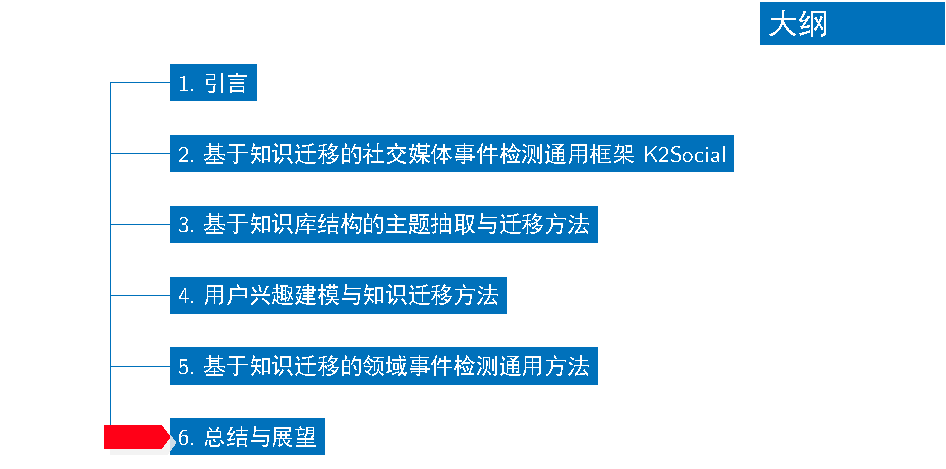
\includegraphics[width=1.0\paperwidth]{img/contents6_output.pdf}
\end{figure}

\end{frame}
\end{withoutheadline}

\section{总结与展望}
%------------------------------
%page 2
\begin{frame}
\frametitle{Motivation}

Many Web applications need the \textbf{accurate event detection} technique on microblog stream, including:
\begin{enumerate}
	%\item 公共舆情分析 [Chen, SIGIR 2013]
	%\item {\kaishu \textbf{公共安全}} [Li, ICDE 2012], [Imran, WWW 2014]
	\item disaster response [Sakaki,WWW 2010]
	\item breaking news report\footnote{\url{http://www.theverge.com/2016/12/1/13804542/reuters-algorithm-breaking-news-twitter}}
\end{enumerate}	
\vfill

But detecting events on twitter stream accurately is still challenging.
\end{frame}

